%%%%%%%%%%%%%%%%%%%%%%%%%%%%%%%%%%%%%%%%%
% University Assignment Title Page 
% LaTeX Template
% Version 1.0 (27/12/12)
%
% This template has been downloaded from:
% http://www.LaTeXTemplates.com
%
% Original author:
% WikiBooks (http://en.wikibooks.org/wiki/LaTeX/Title_Creation)
%
% License:
% CC BY-NC-SA 3.0 (http://creativecommons.org/licenses/by-nc-sa/3.0/)
% 
% Instructions for using this template:
% This title page is capable of being compiled as is. This is not useful for 
% including it in another document. To do this, you have two options: 
%
% 1) Copy/paste everything between \begin{document} and \end{document} 
% starting at \begin{titlepage} and paste this into another LaTeX file where you 
% want your title page.
% OR
% 2) Remove everything outside the \begin{titlepage} and \end{titlepage} and 
% move this file to the same directory as the LaTeX file you wish to add it to. 
% Then add \input{./title_page_1.tex} to your LaTeX file where you want your
% title page.
%
%%%%%%%%%%%%%%%%%%%%%%%%%%%%%%%%%%%%%%%%%
%\title{Title page with logo}
%----------------------------------------------------------------------------------------
%	PACKAGES AND OTHER DOCUMENT CONFIGURATIONS
%----------------------------------------------------------------------------------------

\documentclass[12pt]{article}
\usepackage[english]{babel}
\usepackage[utf8x]{inputenc}
\usepackage{amsmath}
\usepackage{graphicx}
\usepackage[colorinlistoftodos]{todonotes}
\usepackage{url}
\usepackage{tabu}
\usepackage{multirow}

\begin{document}

\begin{titlepage}

\newcommand{\HRule}{\rule{\linewidth}{0.5mm}} % Defines a new command for the horizontal lines, change thickness here

\center % Center everything on the page
 
%----------------------------------------------------------------------------------------
%	HEADING SECTIONS
%----------------------------------------------------------------------------------------

\textsc{\LARGE Université Jean Monnet}\\[1.5cm] % Name of your university/college
\textsc{\Large Data Mining}\\[0.5cm] % Major heading such as course name
\textsc{\large Project Report}\\[0.5cm] % Minor heading such as course title

%----------------------------------------------------------------------------------------
%	TITLE SECTION
%----------------------------------------------------------------------------------------

\HRule \\[0.4cm]
{ \huge \bfseries Meteorite Analysis}\\[0.4cm] % Title of your document
\HRule \\[1.5cm]
 
%----------------------------------------------------------------------------------------
%	AUTHOR SECTION
%----------------------------------------------------------------------------------------

\begin{minipage}{0.4\textwidth}
\begin{flushleft} \large
\emph{Author:}\\
Omar \textsc{Elsabrout} % Your name
\end{flushleft}
\end{minipage}
~
\begin{minipage}{0.4\textwidth}
\begin{flushright} \large
\emph{Supervisor:} \\
Dr. Fabrice \textsc{Muhlenbach} % Supervisor's Name
\end{flushright}
\end{minipage}\\[2cm]

% If you don't want a supervisor, uncomment the two lines below and remove the section above
%\Large \emph{Author:}\\
%John \textsc{Smith}\\[3cm] % Your name

%----------------------------------------------------------------------------------------
%	DATE SECTION
%----------------------------------------------------------------------------------------

{\large \today}\\[2cm] % Date, change the \today to a set date if you want to be precise

%----------------------------------------------------------------------------------------
%	LOGO SECTION
%----------------------------------------------------------------------------------------


\includegraphics[width=60mm]{logo.png}\\[1cm] % Include a department/university logo - this will require the graphicx package
 
%----------------------------------------------------------------------------------------

\vfill % Fill the rest of the page with whitespace

\end{titlepage}


\begin{abstract}
Through out the years, a huge number of meteorites has fallen to Earth from outer space. These incidents are recorded by the Meteoritical Society and stored in a dataset that includes the location, mass, composition, and fall year for over 45,000 meteorites that have struck our planet. Such an interesting topic is perfect to be utilized as a study example for data mining techniques we try to learn in our Data Mining project.
\end{abstract}

\section{Introduction}

Since the objective of the project is to search a real life problem and to find a sufficiently large dataset for being able to apply data mining techniques with \textbf{R} to find some answers to this problem or to extract new strange interesting knowledge out of it. 

A relatively large dataset is selected for the project to find interesting, unexpected or valuable
structures that are embedded in its data. This dataset was downloaded from NASA’s Data Portal, and is based on The Meteoritical Society's Meteoritical Bulletin Database (this latter database provides additional information such as meteorite images, links to primary sources, etc.). The dataset can be downloaded from the following link (\url{https://data.nasa.gov/Space-Science/Meteorite-Landings/ak9y-cwf9})



\section{Problem Understanding}
Concerning the given dataset of meteorite landings, it does not have the regular paradigm of a dataset designed for problem solving. On the other hand, it represents observations of nature and outer space which makes the dataset belong to the category which we only seek to extract some phenomenon or strong correlations. Until now, space still hold several unexplained phenomena and the scientific community has been collecting data for many years to help us mine this knowledge and reach new conclusions.

Getting into understanding what meteorites are, a meteorite is a solid piece of debris from an object, such as a comet, asteroid, or meteoroid, that originates in outer space and survives its passage through the atmosphere to reach the surface of a planet or moon. Meteorites that are recovered after being observed as they transit the atmosphere or impact the Earth are called meteorite falls. All others are known as meteorite finds. As of April 2016, there were about 1,140 witnessed falls that have specimens in the world's collections. As of 2011, there are more than 38,660 well-documented meteorite finds.

One of the features tackled in this report is the type of meteorite recovery. Hence, it is crucial to understand the types of recoveries of meteorites before looking into the dataset. There are two meteorite recovery types which are Falls and Finds. Most meteorite falls are recovered on the basis of eyewitness accounts of the fireball or the impact of the object on the ground, or both. Therefore, despite the fact that meteorites fall with virtually equal probability everywhere on Earth, verified meteorite falls tend to be concentrated in areas with high human population densities such as Europe, Japan, and northern India. A small number of meteorite falls have been observed with automated cameras and recovered following calculation of the impact point. NASA, which is the provider of our dataset, has an automated system that detects meteors and calculates the orbit, magnitude, ground track, and other parameters over the southeast USA, which often detects a number of events each night.

\section{Data Understanding}
One of the most important concerns when it comes to data mining in general is understanding the dataset and its purpose before starting to process it. In our case, we have to understand what are meteorites and their landings which is explained in the previous part. On the other hand, in this section we go more into details regarding the dataset itself. Our dataset is imported from NASA's open data portal in a CSV format to be imported to R studio. Our dataset consists of ten features which are `name', `id', `nametype', `recclass', `mass', `fall', `year', `reclat', `reclong' and `GeoLocation' respectively. The dataset has 45,617 rows accordingly which makes it a great setup for unsupervised learning since we have no labels for each row. 

In order to show our work on the data, a specific explanation for every column has to be presented to understand the purpose of our analysis. In a column by column manner, we start with the most basic feature which is the `name' which basically expresses the name of the meteorite in a string form. Following, the `id' feature which is surprisingly does not depend on the time of discovery of the meteorite and seems to be randomly selected. Nonetheless, it is a valid identification of the meteorite since no two rows have the same `id'. Then, the `nametype' feature which has the value ``Valid'' for all meteorites which is completely useless. However, we might think it is a leftover of another dataset that contained valid and invalid rows and then it got filtered. Next, we have the `recclass' feature which is a text that represents the elements forming this meteorite. This information is valuable from a geological and astrophysical point of view and is helpful to our understanding of the different types of meteorites. Then, one of the most important features is `mass' since it expresses the mass of the meteorite in kilograms. Next, we check the feature `fall' which has only two values either Found or Fall. This indicates the type of meteorite previously explained which contributes significantly to our understanding of the data. Then, the feature `year' shows the time of the landing of the meteorite which is an extremely difficult task if the meteorite is already found on earth. Hence, there are several rows without a value for this feature which is understandable but causes to lower the quality of the data. The following two features are correlated which are `reclat' and `reclong'. They represent the location coordinates of the meteorite which takes us to the following feature. Finally, the last feature is `GeoLocation' which is redundant since it depends completely and only on the `reclat' and `reclong' features without any addition of information.

This concludes the explanation of all of our features and their usefulness. Our next step is to prepare these features and adjust the data in general to start our analysis. Such task is crucial and encouraged as it optimizes the analysis process.


\section{Data Preparation}
Most of available dataset are collected only for the purpose of preserving knowledge. However, that does not mean they are ready for knowledge mining instantly. Several observations and manipulations are in order to extract this knowledge and analyze it. 

In our case, some modifications are done to make the data as expressive as possible. First, we discarded the feature `GeoLocation' since it adds absolutely no new knowledge and it is composed of the `reclat' and `reclong' features. Secondly, we reformat the feature `year' as the rows do not have the same format. Some of them are dates with days, months and years. On the other hand, some of them are only years. We decided that only years are relevant in our analysis. Such process can be done using R in a script but we found that it can be done just as easily in Microsoft Excel without the need to implement a script or code snippet. At the end, only results matter and efficiency dictates that we select the simplest method if we do not sacrifice quality.

At last, we realize that the data is incomplete in several rows due to the fact that it is collected from several entities with different quality measures. Hence, we filter incomplete rows before getting into the analysis process. By filtering we mean removing rows with missing features, rows in invalid years and rows with strange and out of the scope locations. This helps us in reaching solid and reliable results and removes noise from the data.

\section{Modeling and Evaluation}
In our report, we present the mined knowledge in form of sections since modeling in our case is unconventional as a result of observing natural phenomena and not a dedicated dataset to solve a specific problem. The paradigm of our project is different from the conventional form because we had to adapt our prospective to match our dataset.

\subsection{Class Analysis} 
\subsubsection{Meteorite Class Count}
We plot the twenty most occurring meteorites in a flipped bar plot in Figure \ref{fig:fig2}. This indicates which classes are the most frequent.
\begin{figure}
	\centering
	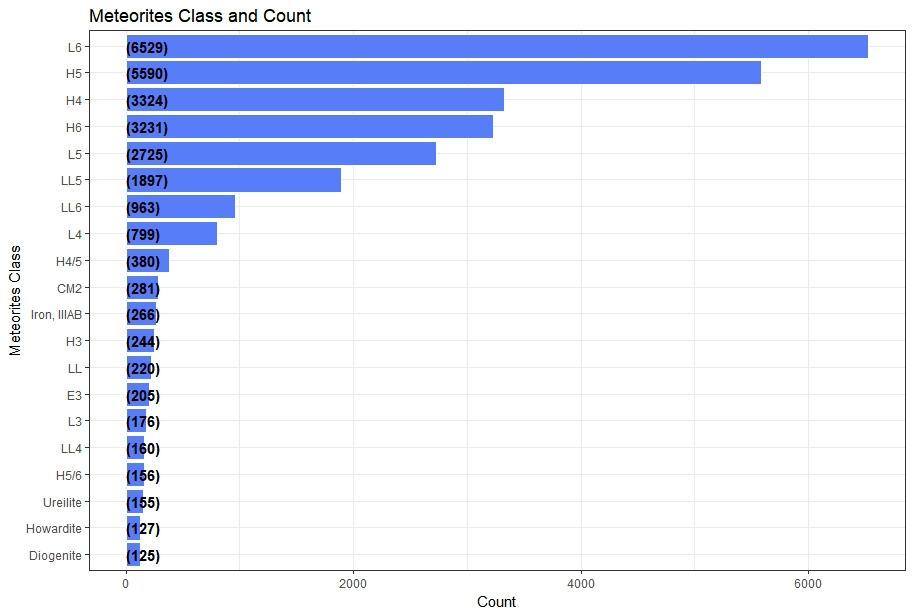
\includegraphics[width=0.9\textwidth]{Figures/02MostOccuring.jpeg}
	\caption{\label{fig:fig2} Meteorites Class and Count.}
\end{figure}

\subsubsection{Meteorite Mass Count}
We plot the twenty most heavy meteorites based on their median mass in a flipped bar plot. in Figure \ref{fig:fig4}. This shows the correlation between meteorite mass and frequency.
\begin{figure}
	\centering
	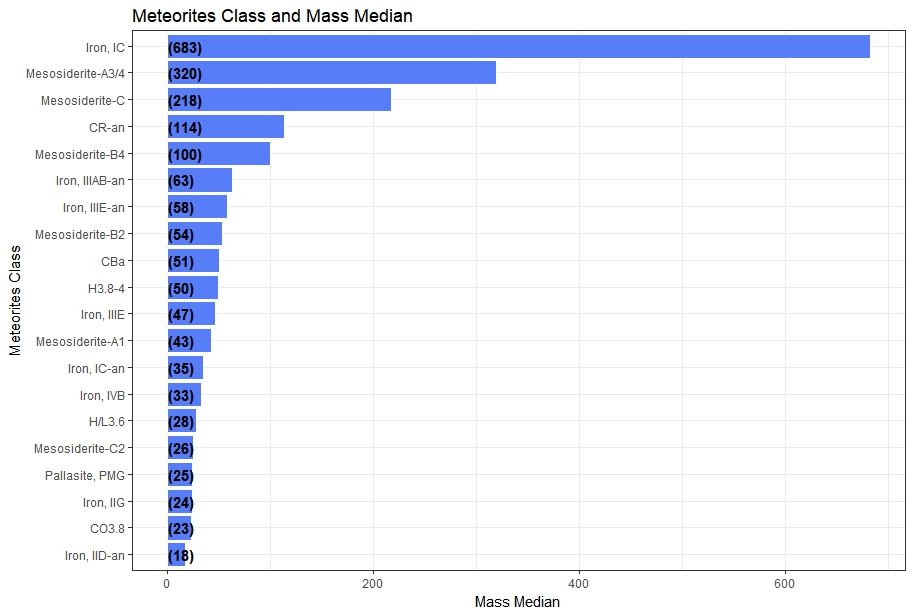
\includegraphics[width=0.9\textwidth]{Figures/04Top20Heaviest.jpeg}
	\caption{\label{fig:fig4} Meteorites Mass and Count.}
\end{figure}

\subsection{Distribution of Mass}
Here Mass is a continous variable and therfore for the distribution we plot a histogram. We plot the distribution of the Mass of the meteorites in Figure \ref{fig:fig6}.
\begin{figure}
	\centering
	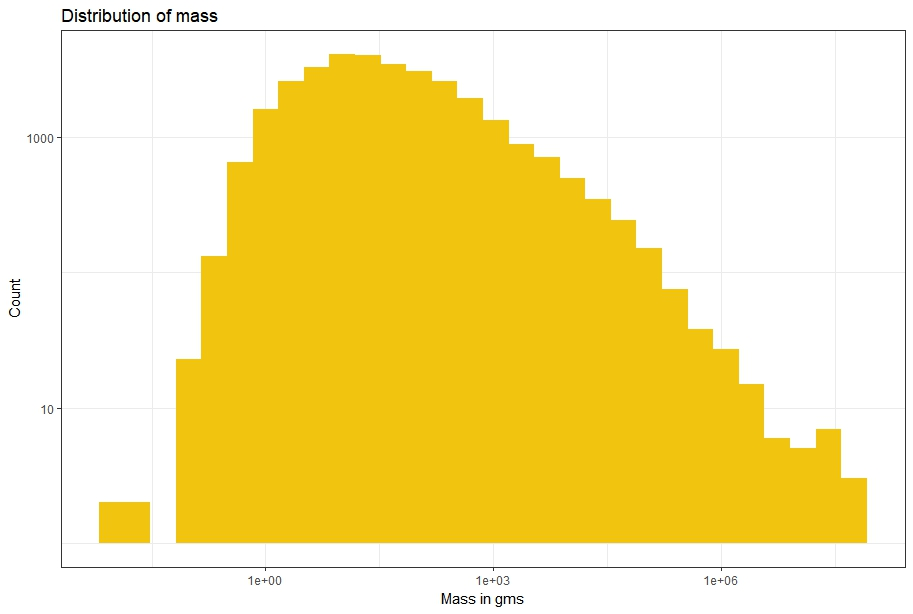
\includegraphics[width=0.9\textwidth]{Figures/06DistributionOfMass.jpeg}
	\caption{\label{fig:fig6} Distribution of Mass.}
\end{figure}

\subsubsection{Heaviest Meteorite}
We extract the heaviest meteorite with its mass is in Kilograms.
\begin{center}
	\centering
	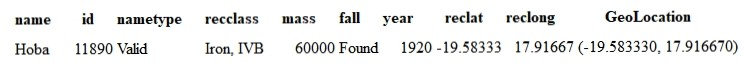
\includegraphics[width=0.9\textwidth]{Figures/07HeaviesMeteorite.jpeg}
\end{center}

\subsubsection{Map of the Heaviest Meteorite}
The mass of the meteorites are indicated by the radius of the circles. The radius is equal to the mass in kilograms multiplied by 10 in Figure \ref{fig:fig8}.
\begin{figure}
	\centering
	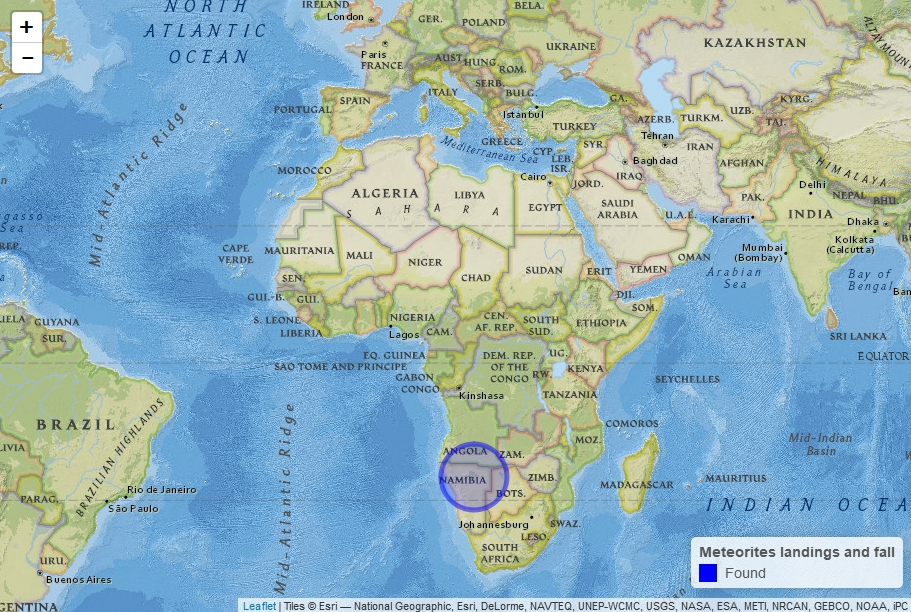
\includegraphics[width=0.9\textwidth]{Figures/08HeaviestMeteorite.jpeg}
	\caption{\label{fig:fig8} Heaviest Meteorite.}
\end{figure}

\subsubsection{Lightest Meteorite}
We extract the lightest meteorite with its mass is in Kilograms.
\begin{center}
	\centering
	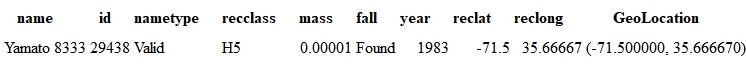
\includegraphics[width=0.9\textwidth]{Figures/10ValidLightestMeteorite.jpeg}
\end{center}

\subsubsection{Distribution of Mass classified by Fall Type}
We plot the distribution of the mass of the meteorites based on their fall type in Figure \ref{fig:fig11}. To examine the relationships between a continuous and categorical variable, we plot a facet bar plot in Figure \ref{fig:fig12}.
\begin{figure}
	\centering
	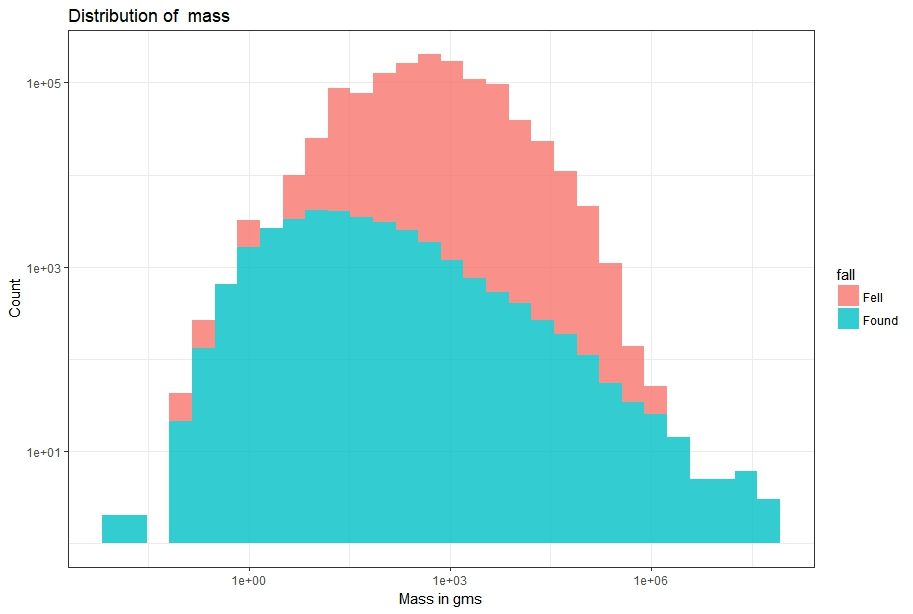
\includegraphics[width=0.9\textwidth]{Figures/11DistributionOfMass.jpeg}
	\caption{\label{fig:fig11} Distribution Of Mass.}
\end{figure}
\begin{figure}
	\centering
	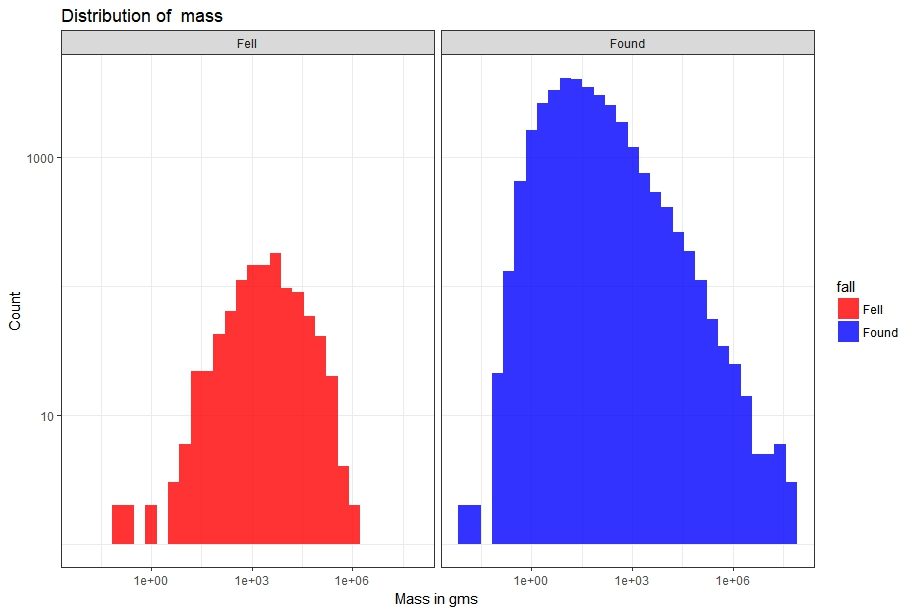
\includegraphics[width=0.9\textwidth]{Figures/12DistributionOfMass.jpeg}
	\caption{\label{fig:fig12}  Distribution Of Mass.}
\end{figure}

\subsection{Distribution of Meteorite Landings with Meteorite Mass}
The following plot shows the distribution of the meteorite landings all over the world. The mass of the Meteorites are indicated by the Radius of the Circles. Plot is shown in Figure \ref{fig:fig14}.
\begin{figure}
	\centering
	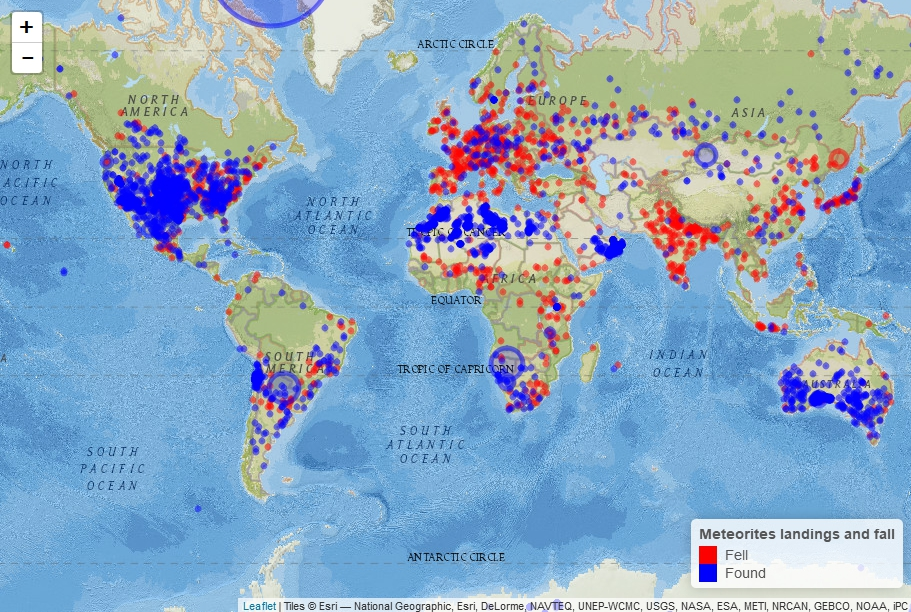
\includegraphics[width=0.9\textwidth]{Figures/14MapOfMeteorites.jpeg}
	\caption{\label{fig:fig14} Map of Meteorites.}
\end{figure}

\subsection{Distribution of US Meteorite Landings}
The following plot shows the distribution of the US meteorite landings.Here we have filtered the US meteorite landings by filtering the latitude and longitude in Figure \ref{fig:fig17}. The heaviest ten of them are represented in the following table:
\begin{center}
	\centering
	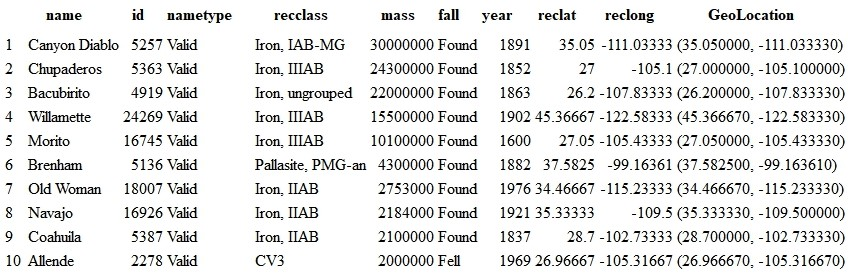
\includegraphics[width=0.9\textwidth]{Figures/16MeteoritesOfUS.jpeg}
\end{center}
\begin{figure}
	\centering
	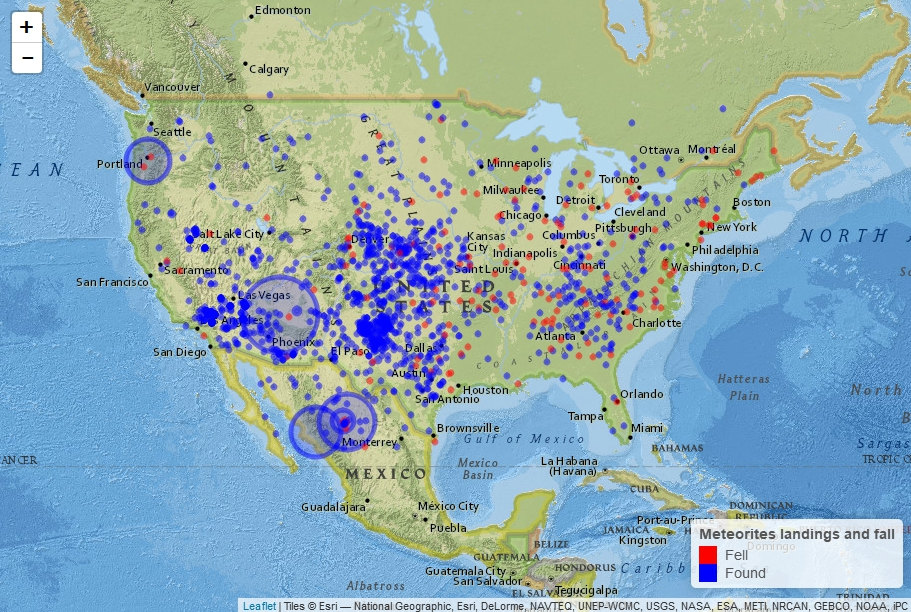
\includegraphics[width=0.9\textwidth]{Figures/17MeteoritesByMassUS.jpeg}
	\caption{\label{fig:fig17} Map of Meteorites by Mass in US.}
\end{figure}

Moreover, we go further into guessing the geographical most probable places to have meteorite landings in the US. These places are represented in a heat map in Figure \ref{fig:fig18}.
\begin{figure}
	\centering
	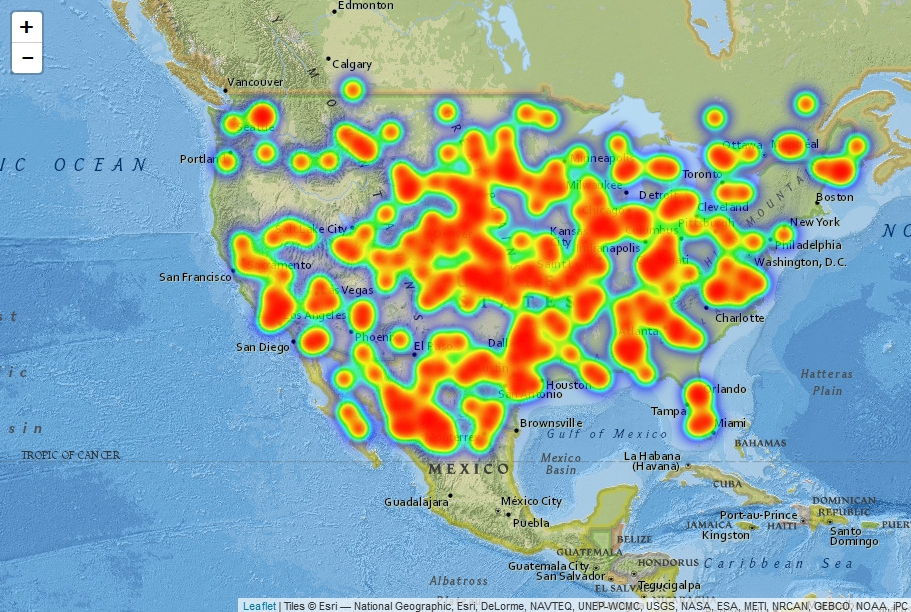
\includegraphics[width=0.9\textwidth]{Figures/18HeatmapUS.jpeg}
	\caption{\label{fig:fig18}  Heat map of the US.}
\end{figure}

Since we consider the US as a sample space of the entire map. We go further into one of the techniques regarding unsupervised learning datasets such as ours. We cluster the meteorite landings in the US and show them over the map to summarize the information in the heat map and provide useful knowledge for future astrophysicists and geologists. The clustering map is shown in Figure \ref{fig:fig19}.
\begin{figure}
	\centering
	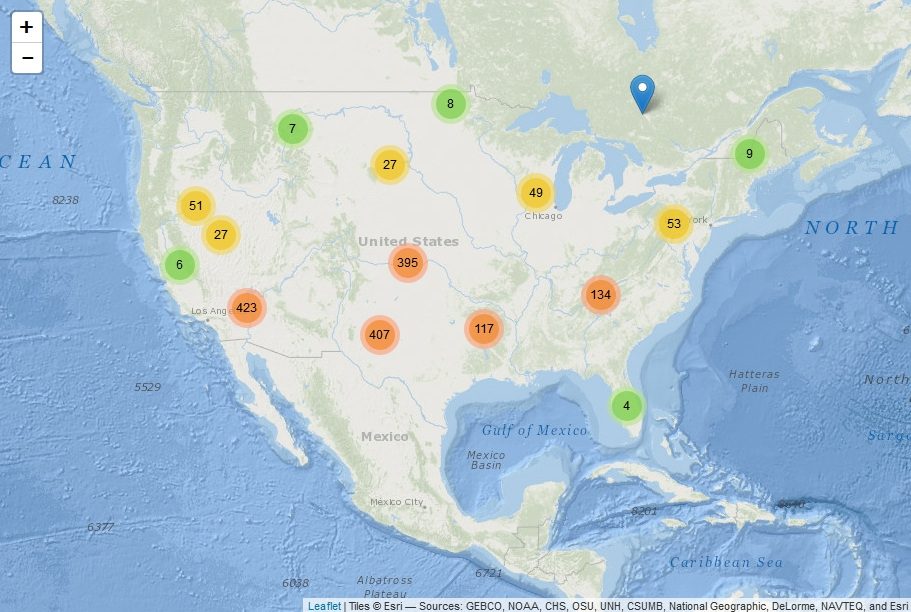
\includegraphics[width=0.9\textwidth]{Figures/19ClusterMarkersUS.jpeg}
	\caption{\label{fig:fig19}  Clustering map of the US.}
\end{figure}

\subsection{Year Analysis}
One of the most popular misconceptions is that meteorite landings are growing bigger in numbers with time which is completely false according to our findings of the dataset and to our Figure \ref{fig:fig20} which indicates that there is absolutely no solid correlation between the count of meteorite landings and time.
\begin{figure}
	\centering
	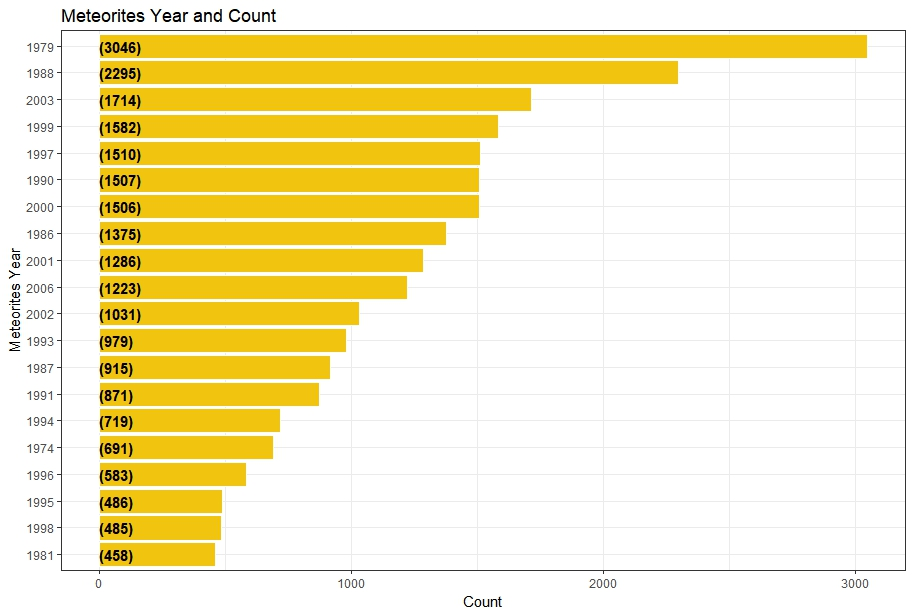
\includegraphics[width=0.9\textwidth]{Figures/20YearAnalysis.jpeg}
	\caption{\label{fig:fig20}  Meteorites Year and Count.}
\end{figure}

\section{Deployment}
This work of analysis is implemented using R and R studio software. Our implementation is written in a single long script with proper commenting to explain the executed operations. Then, we stored the project on a GitHub repository on the the following link: \\
\url{https://github.com/Sabrout/MeteoriteAnalysis}

Surprisingly, it was expected to implement a machine learning algorithm to predict or solve a problem. On the other hand, such idea does not fit natural observations of phenomena in our case which leads us to do more of a data analysis approach to find strong correlations more than a problem solving oriented approach. 

\section{Conclusion}
To sum up, we discovered more knowledge about meteorite landings when we applied data mining techniques. Such knowledge might be a little bit vague at the current time being. Nonetheless, progressing on this analysis with deeper tools and analysis might lead to even more important and more interesting findings. This is considered a milestone for a promising future work. 

%\label{sec:examples}
%
%\subsection{Sections}
%
%Use section and subsection commands to organize your document. \LaTeX{} handles all the formatting and numbering automatically. Use ref and label commands for cross-references.
%
%\subsection{Comments}
%
%Comments can be added to the margins of the document using the \todo{Here's a comment in the margin!} todo command, as shown in the example on the right. You can also add inline comments too:
%
%\todo[inline, color=green!40]{This is an inline comment.}
%
%\subsection{Tables and Figures}
%
%Use the table and tabular commands for basic tables --- see Table~\ref{tab:widgets}, for example. You can upload a figure (JPEG, PNG or PDF) using the files menu. To include it in your document, use the includegraphics command as in the code for Figure~\ref{fig:frog} below.

% Commands to include a figure:
%\begin{figure}
%\centering
%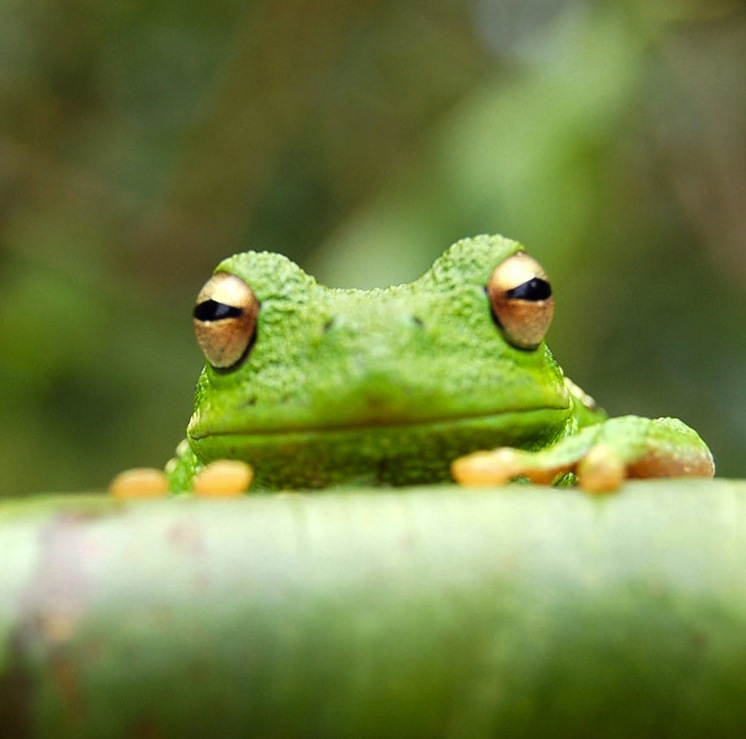
\includegraphics[width=0.5\textwidth]{frog.jpg}
%\caption{\label{fig:frog}This is a figure caption.}
%\end{figure}
%
%\begin{table}
%\centering
%\begin{tabular}{l|r}
%Item & Quantity \\\hline
%Widgets & 42 \\
%Gadgets & 13
%\end{tabular}
%\caption{\label{tab:widgets}An example table.}
%\end{table}
%
%\subsection{Mathematics}
%
%\LaTeX{} is great at typesetting mathematics. Let $X_1, X_2, \ldots, X_n$ be a sequence of independent and identically distributed random variables with $\text{E}[X_i] = \mu$ and $\text{Var}[X_i] = \sigma^2 < \infty$, and let
%$$S_n = \frac{X_1 + X_2 + \cdots + X_n}{n}
%      = \frac{1}{n}\sum_{i}^{n} X_i$$
%denote their mean. Then as $n$ approaches infinity, the random variables $\sqrt{n}(S_n - \mu)$ converge in distribution to a normal $\mathcal{N}(0, \sigma^2)$.
%
%\subsection{Lists}
%
%You can make lists with automatic numbering \dots
%
%\begin{enumerate}
%\item Like this,
%\item and like this.
%\end{enumerate}
%\dots or bullet points \dots
%\begin{itemize}
%\item Like this,
%\item and like this.
%\end{itemize}
%
%We hope you find write\LaTeX\ useful, and please let us know if you have any feedback using the help menu above.
%
\end{document}